\documentclass[a4paper,11pt]{article}
\usepackage[T1]{fontenc}
\usepackage[utf8]{inputenc}
\usepackage{lmodern}
%\usepackage{ngerman}
\usepackage{graphicx}
\usepackage{float}
\usepackage{attachfile}
\usepackage[T1]{fontenc}
%\usepackage{beramono}% monospaced font with bold variant

\usepackage{listings}
\lstdefinelanguage{VHDL}{
  morekeywords={
    library,use,all,entity,is,port,in,out,end,architecture,of,
    begin,and,generic,process,if,then,elsif,else,when,
    signal, integer,std_logic,unsigned,signed,std_logic_vector,
    constant, variable, wait, for, until, map
  },
  morecomment=[l]--
}

\usepackage{xcolor}
\colorlet{keyword}{blue!100!black!80}
\colorlet{comment}{green!90!black!90}
\lstdefinestyle{vhdl}{
  language     = VHDL,
  basicstyle   = \ttfamily\scriptsize,
  keywordstyle = \color{keyword}\bfseries,
  commentstyle = \color{comment}
}

\lstdefinestyle{c}{
  language     = c,
  basicstyle   = \ttfamily\scriptsize,
  keywordstyle = \color{keyword}\bfseries,
  commentstyle = \color{comment}
}

\usepackage{hyperref}  %remove the red boxes at contents
\hypersetup{colorlinks=true,linkcolor=black}

\usepackage{fancyvrb}

\setlength{\parindent}{0em} 


\title{How to simulate an UART VHDL code with ghdl}
\author{René Doß \\ info@dossmatik.de}

\begin{document}

\maketitle
\tableofcontents

\begin{abstract}
This article was written to demonstrate on a practical example how ghdl works. The reader should have basic knowledge about VHDL. This example is fitable code into a FPGA. The code is written vendor independent. UART as example is generally understandable and also parctical on many applications.
An asynchronous serial transmission has two parts Receiver and Transmitter. The handling is typical integrated on all microcontrollers today. Different sensors can communicate over UART. This makes this data transmission very interesting for a hardware developer. The Receiver and Transmitter code is included with an integrated FIFO. These all are demonstrated with ghdl simulation. You will get new spirit for VHDL code validation. The VHDL files are attached in this document.
\end{abstract}

\newpage
\section{introduction UART transmission}
The signal is at silence condition high. A low on line manifests a start of transmission, followed by a number of data bits. The data bits are send from least significant bit (LSB) to most significant bit (MSB). Next bit is a high, witch is called stop bit and it is needed to mark the end of transmission. In this state a new start bit can be correct capture by the receiver. Note that no clock signal has sent through the serial line. The transmitter resynchronize on the falling edge in start bit condition. The data speed and the data length of sender an receiver have to be the same.
\begin{figure}[H]
  \begin{center}
    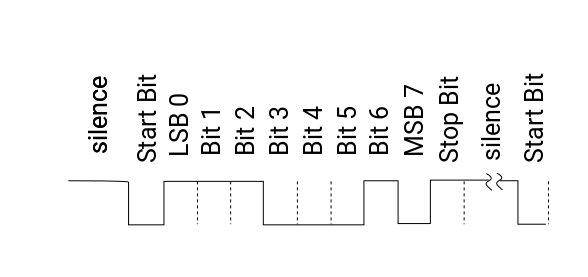
\includegraphics[scale=0.5]{UART_timing.png}
    \caption{UART Timing}
    \label{fig:UART Timing}
  \end{center}
\end{figure}

The baudrate specifies the transmission speed. The unit is baud bit per second.  Common baudrates are established. 
Internally the hardware of UART runs in higher clock rate.

\section{advanced TX Unit with FIFO}
The UART interface is slow and needs a buffer for better synchronisation. Data is written in a FIFO. FIFO is the abrivation first in first out. This FIFO is realised in a ring buffer. Figure \ref{fig:FIFO pointer} explains how it works. Two pointers point at an address of internal RAM. The pointer nextwrite points to the address where the next incoming data will be written. When new data is incoming the FIFO the pointer is increased. Now valid data has to be read from the FIFO  and the nextread is increased. If the two pointers in the FIFO are equal the FIFO is empty.

\begin{figure}[H]
  \begin{center}
    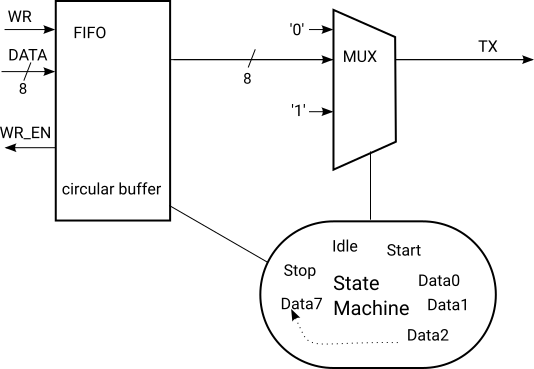
\includegraphics[scale=0.5]{tx/BlockTX.png}
    \caption{Blockdiagram TX}
    \label{fig:Blockdiagram}
  \end{center}
\end{figure}
\hrule
\lstinputlisting[style=vhdl]{tx/UART_TX_8N1.vhd}
\hrule
\vspace{10pt}
\begin{figure}[H]
  \begin{center}
    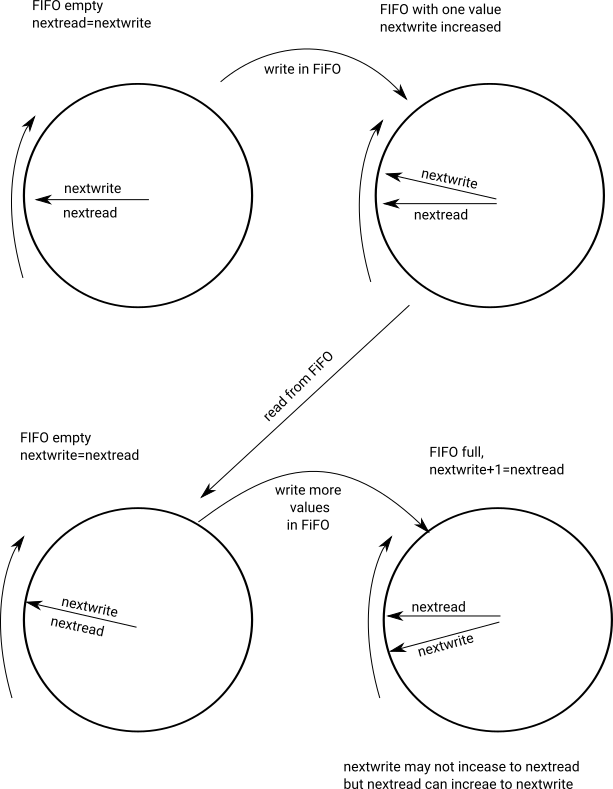
\includegraphics[scale=0.4]{tx/path6054.png}
    \caption{FIFO pointer}
    \label{fig:FIFO pointer}
  \end{center}
\end{figure}
 The FIFO is a circular buffer and works with two address pointers. One pointer is used to point at the write address. The other pointer points at the read address. Both pointers are increased with one step. The interface has two control signals for handshakes. send\_busy and send\_empty these are the FIFO states full and empty. The distance between nextwrite and nextread generates the signal busy because even one more wirte action would cause an overflow in the buffer.
 The testbench is required.
\\
\hrule
\lstinputlisting[style=vhdl]{tx/tb_UART_TX_8N1.vhd}
\hrule
\vspace{10pt}
Put both files in the same directory and simulate this testcase and check the timing requirements.

\begin{verbatim}
ghdl -i *.vhd
ghdl -m tb_UART_TX_8N1
ghdl -r tb_UART_TX_8N1 --stop-time=200us --wave=TX.ghw
gtkwave TX.ghw
\end{verbatim}

\begin{figure}[H]
  \begin{center}
    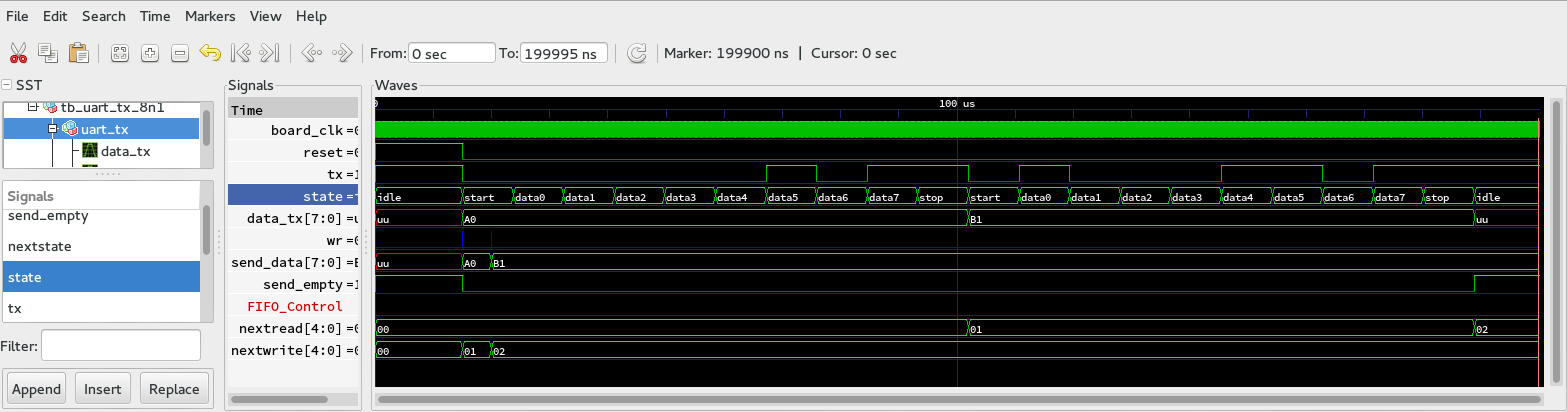
\includegraphics[scale=0.3]{tx/TX_simple.png}
    \caption{UART TX output}
  \end{center}
\end{figure}

\section{advanced RX Unit with FIFO}
The receiver is the opposite component of the transmitter. The code is mapped also in this article. The generic is used to set the right timing. The tick\_counter is the timer of one bit. The counter range of tick is calculated by the generic clk\_freq and baudrate. These parameters make the code portable into different designs. There is nothing to change inside the code when another frequency or baudrate are used. Such parameter makes source code simpiler reusable. When the transmission is off, the RX has a high on line. The state maschine is in idle and waits for RX to turn low. This condition is checked of the falling edge on the start bit. All other bits are cought in the middle of the bit time. 
\\
\hrule
\lstinputlisting[style=vhdl]{rx/UART_RX_8N1.vhd}
\hrule
\vspace{10pt}
Now the apposite testbench.
\hrule
\lstinputlisting[style=vhdl]{rx/tb_UART_RX_8N1.vhd}
\hrule
\vspace{10pt}

\begin{verbatim}
ghdl -i *.vhd
ghdl -m tb_UART_RX_8N1
ghdl -r tb_UART_RX_8N1 --stop-time=800us --wave=RX.ghw
gtkwave RX.ghw
\end{verbatim}

\begin{figure}[H]
  \begin{center}
    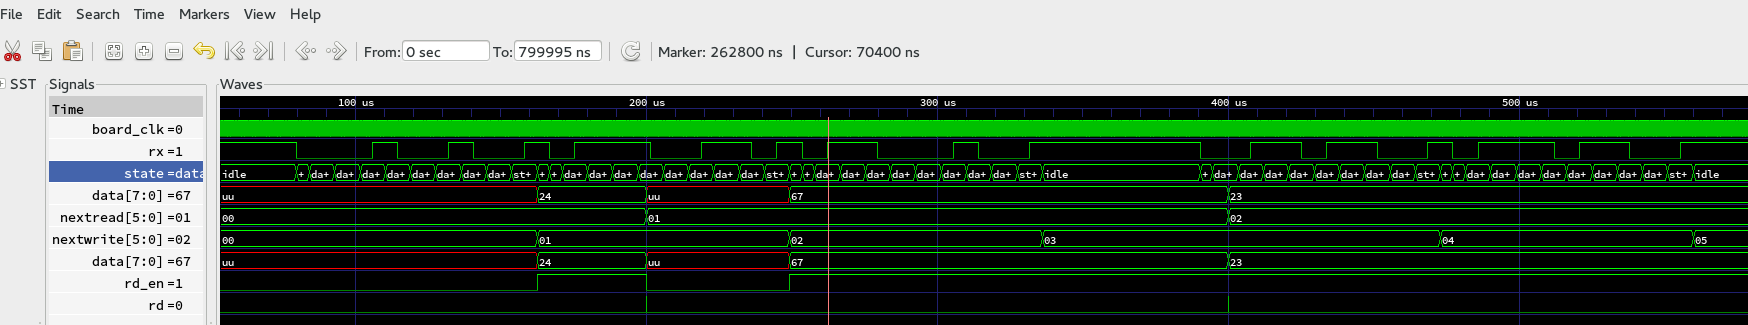
\includegraphics[scale=0.3]{rx/sim_RX.png}
    \caption{UART RX in}
    \label{fig:sim RX}
  \end{center}
\end{figure}

\section{example application}
In the last sections we have designed an input and an output interface. By combinating the receiving and transmitting example, we can build the full UART. Now let us make a simple capitalisation ASCII engine. This is more a theoretical example for a demonstration. The data stream is very simple. It demonstrates how it works.
\\
\hrule
\lstinputlisting[style=vhdl]{capitalisation/capitalisation.vhd}
\hrule
\vspace{10pt}

The application has an 8bit input and a 8bit output interface. A top instance combine the application and the RX und TX interface together. RX and TX are the physical wires and board\_clk is the internal clock of all. This design is competent to fit inside an FPGA. 
\begin{figure}[H]
  \begin{center}
    \includegraphics[scale=0.4]{capitalisation/zeichnung.png}
  \end{center}
\end{figure}

\hrule
\lstinputlisting[style=vhdl]{capitalisation/top_capitalisation.vhd}
\hrule
\vspace{10pt}
Also for this the testbench.
\\
\hrule
\lstinputlisting[style=vhdl]{capitalisation/tb_capitalisation.vhd}
\hrule
\vspace{10pt}

\begin{figure}[H]
  \begin{center}
    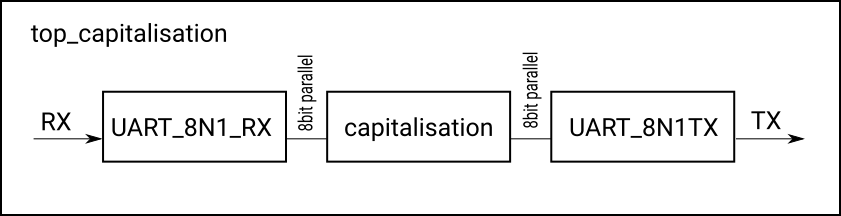
\includegraphics[scale=0.4]{capitalisation/capitalisation.png}
    \caption{capitalisation}
    \label{fig:capitalisation}
  \end{center}
\end{figure}

\section{Makefile for workflow}
Make is a build tool from the GNU Project. Mostly it is used to control compiling a huge number of files ans solve dependencies. For simplify your life and enhance your productivity you can use is also the make tool to prepair the target in the ghdl simulation. The makefile is like a script with sequential commands. Sometimes rules are insert. If you have larger designs, you should also divide the VHDL design into different files. I use \textbf{make} for this. Store the makefile into the same folder. For run in GHDL type make, this starts all commandos under all. And for view inside the timingdiagram type \textbf{make view}. You find many examples but I give you my makefile for a simple start in GHDL application.
\\
\hrule
\VerbatimInput{capitalisation/makefile}
\hrule
\vspace{10pt}


\section{file in/out}
In former section we had simulate the whole desgin. In larger designs this can be difficult. It needs time to run and it can be also possible some parts are not read. You have to divide the design in moduls and you have to test the moduls by itselfs. Tested moduls can be integated inside the design. The simple 8bit interface is an good standard. Now I show you. How a module can be tested with datas from an file and also put the output into a file. Sometimes is this simpiler to check as a view in a timing diagram. 
\begin{figure}[H]
  \begin{center}
    \includegraphics[scale=0.4]{file_in_out/zeichnung.png}
  \end{center}
\end{figure}
The file \textbf{test.txt} is read and the characters  goes into the capitalisation and are written in the file \textbf{text1.txt}. 

\vspace{10pt}
\\
\hrule
\lstinputlisting[style=vhdl]{file_in_out/tb_file.vhd}
\hrule
\vspace{10pt}

\begin{verbatim}
[test.txt]
Hallo world! Can you see my text?
\end{verbatim}

\begin{verbatim}
[test1.txt]
HALLO WORLD! CAN YOU SEE MY TEXT?
\end{verbatim}
VHDL has only restricted file operations. It is not possible to seek the fileposition.

\section{VHPI Interface to an other language}
Here I show one of the highest feature of GHDL. It is possible to link code from another language into the simulation. This can be used for a model or an interface to a real hardware. The possible speed is lower as in an FPGA. For testing is this a change to use mor realistic posibilities. You can data interchange of other programs, for instance testing software. In our case the simulation can communicate with a comport emulator. Linux has pseudoterminals witch is a serial interface in driver lowlever exchange of programs. 
First start the c source file. There are only some c functions.
\begin{figure}[H]
  \begin{center}
    \includegraphics[scale=0.4]{vhpi/zeichnung.png}
  \end{center}
\end{figure}
\vspace{10pt}
\\
\hrule
\lstinputlisting[style=c]{vhpi/tty.c}
\hrule
\vspace{10pt}

This package is the glue between external code. All c functions get a wrap of a vhdl definition. That makes possible to call a c function in vhdl. This is the advantage of this VHPI interface.
\vspace{10pt}
\hrule
\lstinputlisting[style=vhdl]{vhpi/tty_pkg.vhd}
\hrule
\vspace{10pt}
Also for that case the testbench.
\vspace{10pt}
\\
\hrule
\lstinputlisting[style=vhdl]{vhpi/tb_tty.vhd}
\hrule
\vspace{10pt}
And the makefile that you can compile and link all together.
\hrule
\VerbatimInput{vhpi/makefile}
\hrule
\vspace{10pt}
In action the simulation prints out the name of the pseudotherminal. I can open a serial terminal program and send datas to the simulation and can also receive the output.

\begin{figure}[H]
  \begin{center}
    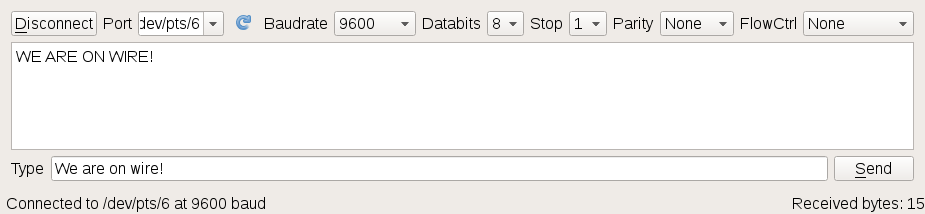
\includegraphics[scale=0.5]{vhpi/terminal.png}
  \end{center}
\end{figure}

\section{closing words}
 The chapter of testbench is very short in the most books. In this article you see the code for testing is adequate to code of application. A simulation is irrecoverable for good results. The development is only effective with simulation. Debug at a later development phase is very difficult. The testbench is the pusher for all effects. The code should also be reusable code. The generic is an interface to set some parameter for a simpler practical integration in the whole application. I hope you could follow all demonstrations and give you idea for better work. 
 
 \begin{verbatim}
  the procedure tx_char was posted of Lothar Miller on
  http:\\www.mikrocontroller.net
  
  the VHPI interface for pseudotherminal was posted 
  of Wojciech M. Zabolotny on comp.arch.FPGA 2011
 \end{verbatim} 

\end{document}
